\documentclass[journal=jpcbfk,manuscript=article]{achemso}

\usepackage[version=3]{mhchem}
\usepackage[T1]{fontenc}
\newcommand*\mycommand[1]{\texttt{\emph{#1}}}
%\newcommand{\todo}[1]{\textcolor{red}{#1}}
\usepackage[obeyFinal]{easy-todo}
\usepackage{rotating}
\usepackage{upgreek}				
\usepackage{xcolor}
\usepackage{booktabs}
\usepackage{multirow}
\usepackage{lmodern}
\usepackage{microtype}
\usepackage{xr-hyper}
\usepackage{soul} % for highlights with \hl{} 
\usepackage{hyperref} % to make TOC titles clickable
\hypersetup{
    colorlinks=true, %set true if you want colored links
    linktoc=all,     %set to all if you want both sections and subsections linked
    linkcolor=black,  %choose some color if you want links to stand out
    citecolor=black,
    filecolor=black,
    urlcolor=black
}

\makeatletter
\newcommand*{\addFileDependency}[1]{% argument=file name and extension
  \typeout{(#1)}
  \@addtofilelist{#1}
  \IfFileExists{#1}{}{\typeout{No file #1.}}
}
\makeatother

\newcommand*{\myexternaldocument}[1]{%
    \externaldocument{#1}%
    \addFileDependency{#1.tex}%
    \addFileDependency{#1.aux}%
}

\myexternaldocument{manuscriptPGPEsuppl}


\author{Am{\'e}lie Bacle}
\affiliation{\tiny Laboratoire Coop{\'e}ratif "Lipotoxicity and Channelopathies - ConicMeds", Universit{\'e} de Poitiers, 1 rue Georges Bonnet, 86000 Poitiers, France }

\author{Pavel Buslaev}
\affiliation{Nanoscience Center and Department of Chemistry, University of Jyv{\"a}skyl{\"a}, P.O. Box 35, 40014 Jyv{\"a}skyl{\"a}, Finland}
\affiliation{Research Center for Molecular Mechanisms of Aging and Age-related Diseases, Moscow Institute of Physics and Technology, 141701 Dolgoprudny, Russia}

\author{Rebeca Garc{\'i}a Fandi{\~n}o}
\affiliation{Center for Research in Biological Chemistry and Molecular Materials (CiQUS), Universidade de Santiago de Compostela, E-15782 Santiago de Compostela, Spain}
\affiliation{CIQUP, Centro de Investigação em Qu{\'i}mica, Departamento de Qu{\'i}mica e Bioqu{\'i}mica, Faculdade de Ci{\^e}ncias, Universidade do Porto, Porto, Portugal}

\author{Fernando Favela-Rosales}
\affiliation{Departamento de Ciencias B\'{a}sicas, Tecnol\'{o}gico Nacional de M\'{e}xico - ITS Zacatecas Occidente, M\'{e}xico}

\author{Tiago M. Ferreira}
\affiliation{NMR group - Institute for Physics, Martin Luther University Halle-Wittenberg, 06120 Halle (Saale), Germany}

\author{Patrick F.J. Fuchs}
\affiliation{Sorbonne Universit{\'e}, Ecole Normale Sup{\'e}rieure, PSL University, CNRS, Laboratoire des Biomol{\'e}cules (LBM), 75005 Paris, France}
\affiliation{Universit{\'e} de Paris, UFR Sciences du Vivant, 75013, Paris, France}

\author{Ivan Gushchin}
\affiliation{Research Center for Molecular Mechanisms of Aging and Age-related Diseases, Moscow Institute of Physics and Technology, 141701 Dolgoprudny, Russia}

\author{Matti Javanainen}
\affiliation{Institute of Organic Chemistry and Biochemistry of the 
Czech Academy of Sciences, Flemingovo n\'{a}m. 542/2, CZ-16610 Prague 6, Czech Republic}

\author{Anne M. Kiirikki}
\affiliation{Institute of Biotechnology, University of Helsinki}


\author{Jesper J. Madsen}
\affiliation{Department of Chemistry, The University of Chicago, Chicago, Illinois, United States of America}
\affiliation{Global and Planetary Health, College of Public Health, University of South Florida, Tampa, Florida, United States of America}

\author{Josef Melcr}
\affiliation{Groningen Biomolecular Sciences and Biotechnology Institute 
and The Zernike Institute for Advanced Materials, 
University of Groningen, 9747 AG Groningen, The Netherlands}

\author{Paula Mil{\'a}n Rodr{\'i}guez}
\affiliation{Sorbonne Universit{\'e}, Ecole Normale Sup{\'e}rieure, PSL University, CNRS, Laboratoire des Biomol{\'e}cules (LBM), 75005 Paris, France}

\author{Markus S. Miettinen}
\affiliation{Department of Theory and Bio-Systems, Max Planck Institute of Colloids and Interfaces, 14424 Potsdam, Germany}
% \affiliation[Max Planck Institute of Colloids and Interfaces]{Department of Theory and Bio-Systems, Max Planck Institute of Colloids and Interfaces, 14424 Potsdam, Germany}


\author{O. H. Samuli Ollila}
\email{samuli.ollila@helsinki.fi}
\affiliation{Institute of Biotechnology, University of Helsinki}

\author{Chris G. Papadopoulos}
\affiliation{Universit{\'e} Paris-Saclay, CEA, CNRS, Institute for Integrative Biology of the Cell (I2BC), 91198 Gif-sur-Yvette, France}


\author{Antonio Pe{\'o}n}
\affiliation{CIQUP, Centro de Investigação em Qu{\'i}mica, Departamento de Qu{\'i}mica e Bioqu{\'i}mica, Faculdade de Ci{\^e}ncias, Universidade do Porto, Porto, Portugal}


\author{Thomas J. Piggot}
\affiliation{Chemistry, University of Southampton, Highfield, Southampton SO17 1BJ, United Kingdom}

\author{{\'A}ngel Pi{\~n}eiro}
\affiliation{Departamento de F{\'i}sica Aplicada, Facultade de F{\'i}sica, Universidade de Santiago de Compostela, E-15782 Santiago de Compostela, Spain}

\author{Salla I. Virtanen}
\affiliation{Institute of Biotechnology, University of Helsinki}


\title{Inverse conformational selection in lipid-protein binding} %Title of paper

\begin{document}

\begin{tocentry}

     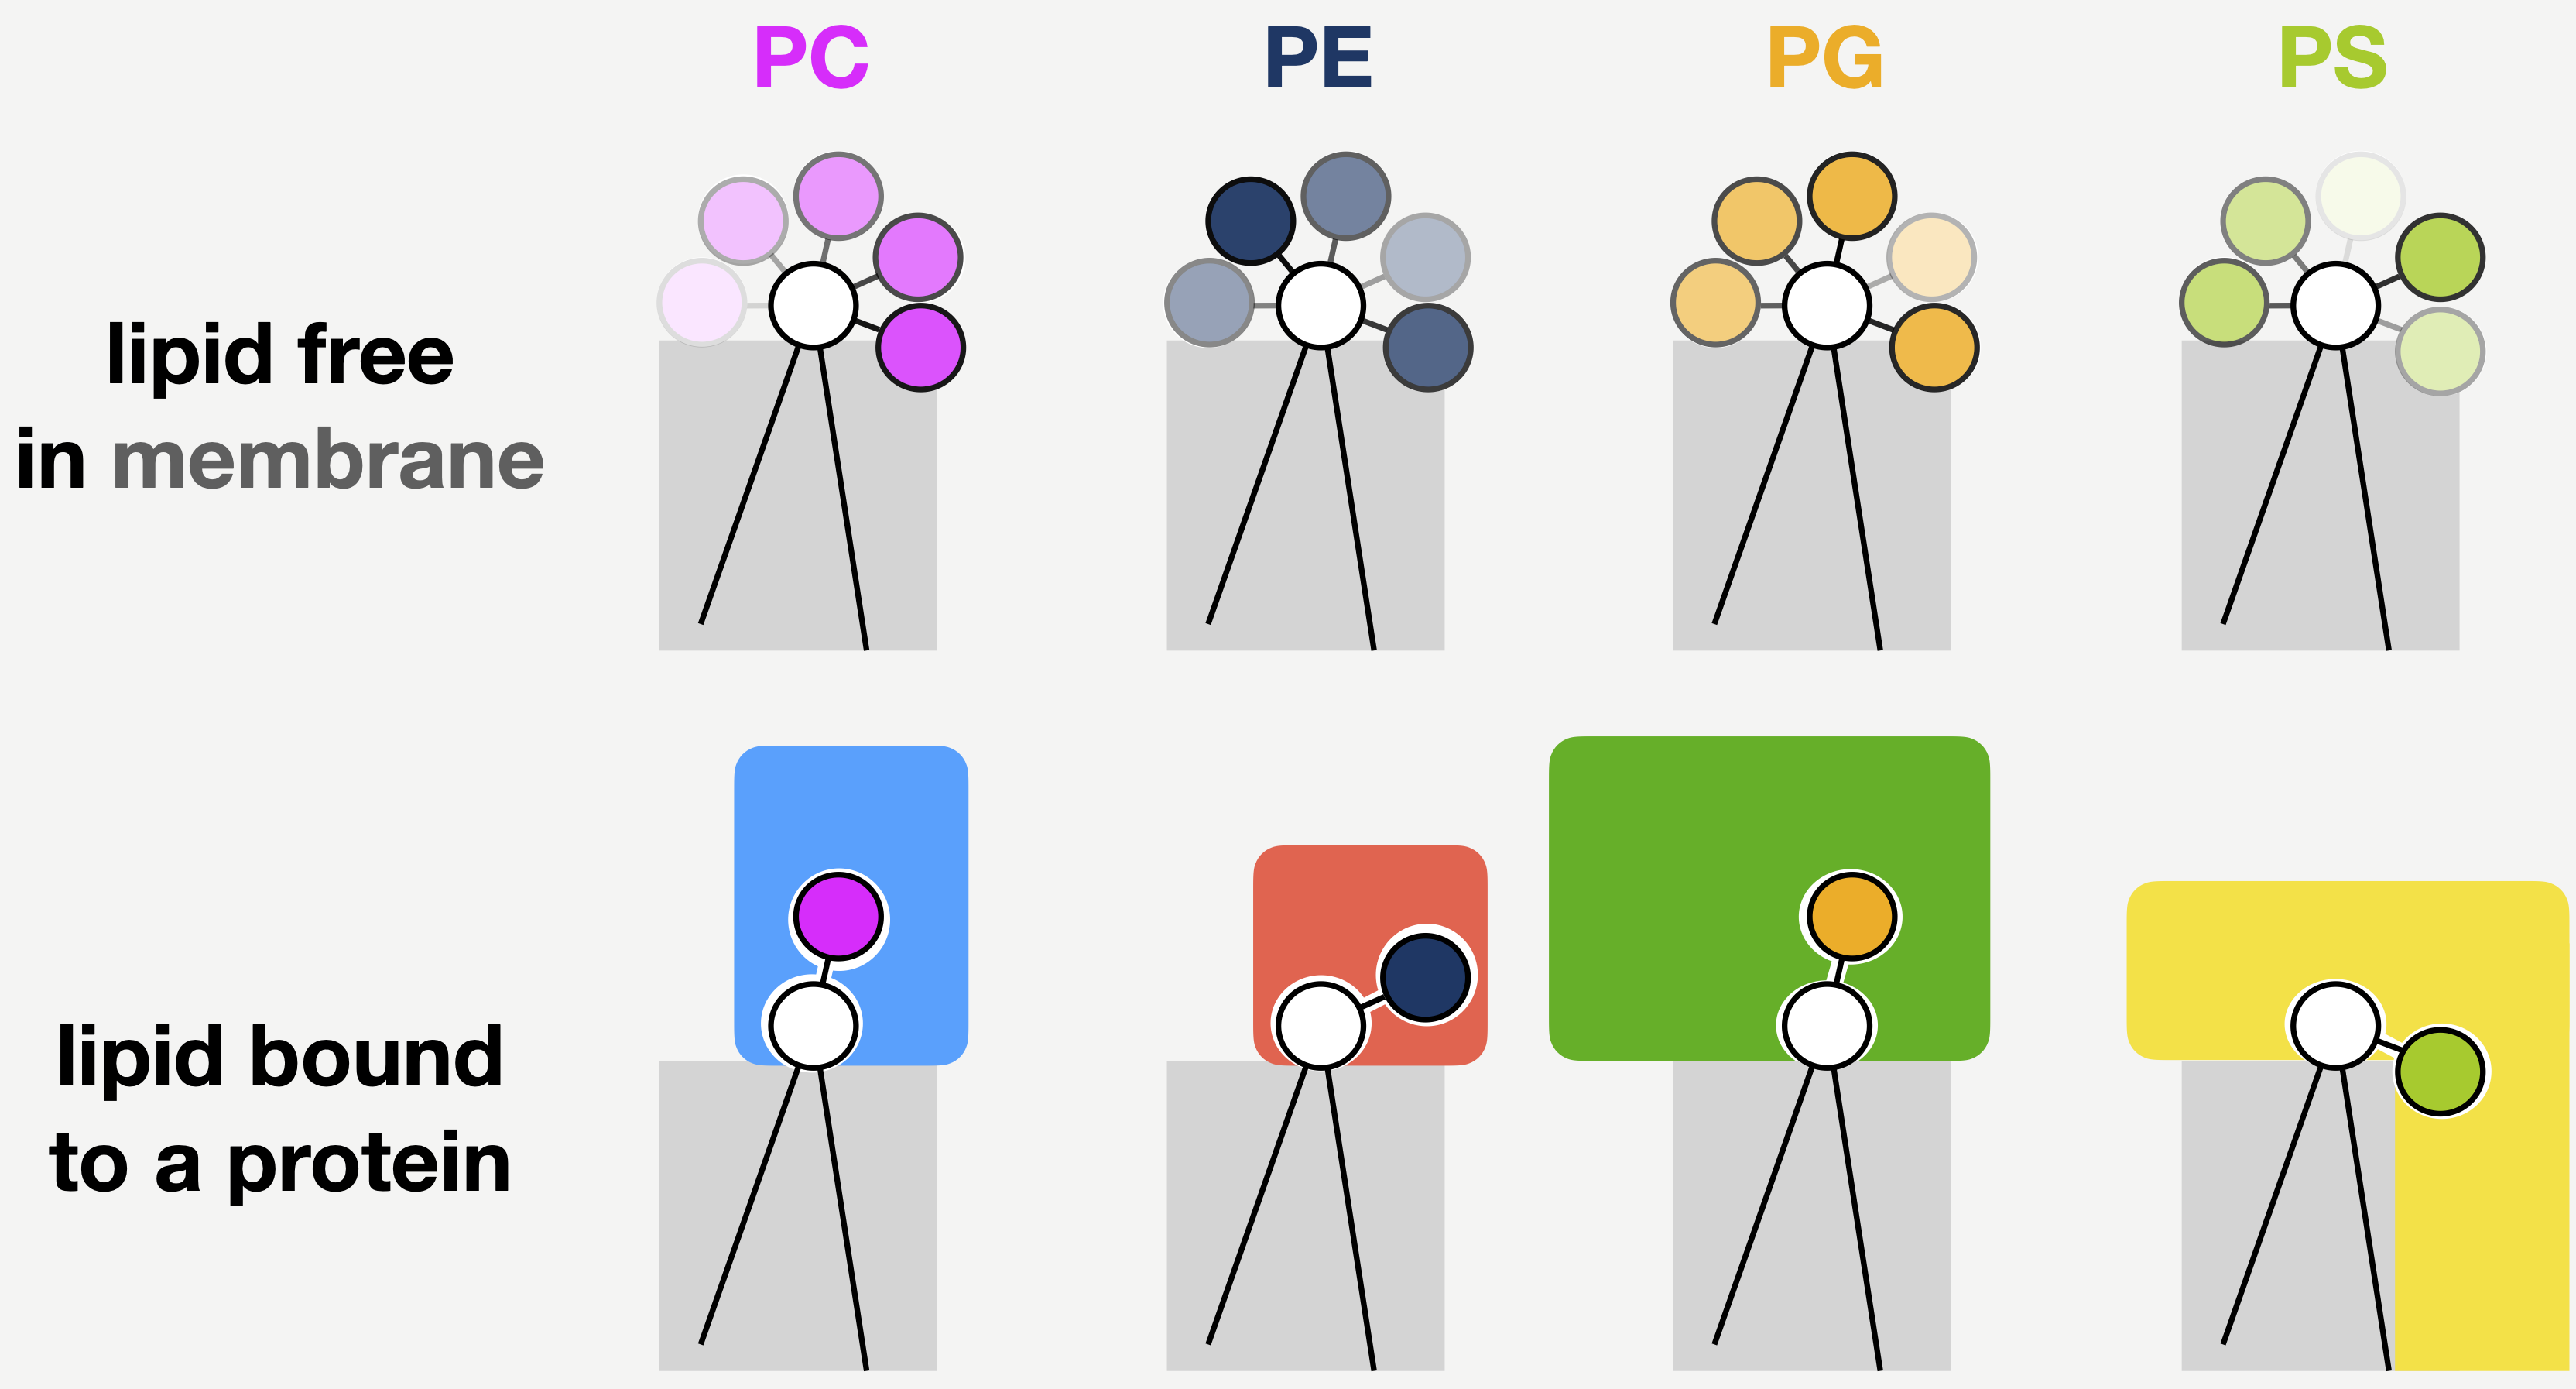
\includegraphics[height=3.5cm]{./Figs/TOC3.png}
%Some journals require a graphical entry for the Table of Contents.
%This should be laid out ``print ready'' so that the sizing of the
%text is correct.

%Inside the \texttt{tocentry} environment, the font used is Helvetica
%8\,pt, as required by \emph{Journal of the American Chemical
%Society}.

%The surrounding frame is 9\,cm by 3.5\,cm, which is the maximum
%permitted for  \emph{Journal of the American Chemical Society}
%graphical table of content entries. The box will not resize if the
%content is too big: instead it will overflow the edge of the box.

%This box and the associated title will always be printed on a
%separate page at the end of the document.

\end{tocentry}


\begin{abstract}
% insert abstract here
  Interest in lipid interactions with proteins and other biomolecules is emerging not only in
  fundamental biochemistry, but also in the field of nanobiotechnology where lipids
  are commonly used, for example, in carriers of mRNA vaccines.
  The outward facing components of cellular membranes and lipid nanoparticles, the lipid headgroups, regulate membrane 
  interactions with approaching substances, such as proteins, drugs, RNA or viruses.
  Because lipid headgroup conformational ensembles  
  have not been experimentally determined in physiologically relevant conditions, an essential question on their interactions with other biomolecules remains unanswered: 
  Do headgroups exchange between a few rigid structures,
  or fluctuate freely across a practically continuous spectrum of  conformations?
  Here, we combine solid-state NMR experiments and molecular dynamics simulations from the NMRlipids Project to resolve the conformational ensembles of headgroups of four key lipid types in various biologically relevant conditions. We find that lipid headgroups sample a wide range of
  overlapping conformations
  in both neutral and charged cellular membranes, and that differences in the headgroup chemistry manifests only
  in probability distributions of conformations. Furthermore,
  the analysis of 894 protein-bound lipid structures from the Protein Data Bank (PDB)
  suggests that lipids can bind to proteins in wide range of conformations,
  which are not limited by the headgroup chemistry.
  We propose that lipids can select a suitable headgroup conformation
  from the wide range available to them to fit the various binding sites in proteins.
  The proposed {\it Inverse Conformational Selection Model} will extend also to lipid binding
  to other targets than proteins, such as drugs, RNA and viruses.

  
\end{abstract}


\maketitle


\section{Introduction}

Lipid interactions with other biomolecules are gaining interest
not only in molecular cell biology \cite{harayama18}, but also in
nanobiotechnology applications, such as design of antibodies \cite{vigant15}
and carriers for mRNA vaccines \cite{pardi18,schoenmaker21}.
Interactions of cellular membranes or lipid nanoparticles with other biomolecules,
such as proteins, drugs or RNA, are regulated by lipid headgroups,
the outward facing components of lipid bilayers \cite{harayama18,vanmeer08}.
Chemical compositions of lipid headgroups vary between different
organelles and organisms, and specific interactions with certain lipid headgroups
are known to be essential for the function of several proteins \cite{harayama18,vanmeer08}.
However, the driving forces for specific interactions between lipids and membrane binding
substances are not fully understood because conformational ensembles of lipids in
physiologically relevant liquid state have not been experimentally determined.
Therefore, it is not clear if the specificity arises from the
differences in accessible conformations between lipid types or
from specific intermolecular lipid--protein interactions.

Structures of protein-bound lipids are available in the Protein Data Bank (PDB, \url{http://www.rcsb.org/}) \cite{berman00},
and crystal structures of lipids have been determined \cite{buldt81,pascher92},
but their relation to lipids in bulk membranes in the liquid lamellar phase remains unclear \cite{marsh13b}. Similarly to disordered proteins~\cite{sormanni17}, lipid molecules sample conformational ensembles that are composed of sets of individual structures whose occurrence probabilities are determined by the Boltzmann distribution~\cite{buslaev16}. In liquid bilayer state, individual phosphatidylcholine lipid samples the conformational ensemble on nanosecond timescale~\cite{ferreira15,antila21a}. The most accurate experimental information on conformational ensembles of lipids
in this biologically relevant phase are typically derived from NMR experiments, particularly from the
C--H bond order parameters, $S_\mathrm{CH}=\frac{1}{2} \langle 3\cos^2 \theta -1 \rangle$, where $\theta$ is the angle between C-H bond and membrane normal, and the average is taken over the conformational ensemble of lipids~\cite{seelig77c,davis83,Semchyschyn04}.
Because these order parameters are similar to those in living cells \cite{gally81,scherer87,seelig90},
the model membranes can be used to resolve the lipid headgroup conformations in biological conditions.
According to these experiments, the glycerol backbone conformations are largely similar irrespective of the headgroup \cite{gally81}, and
the headgroup conformations are similar in the phosphatidylcholine (PC), phosphatidylethanolamine (PE), and phosphatidylglycerol (PG) lipids,
whereas the phosphatidylserine (PS) headgroup is more rigid \cite{wohlgemuth80,buldt81}. 
Notably, however, the signs of $S_\mathrm{CH}$ are not accessible from $^2$H\,NMR experiments \cite{ollila16},
and universal models to map order parameters to structural ensembles are not available \cite{pezeshkian18,akutsu20}.
Therefore, it is not clear if the lipid headgroups in a liquid lamellar bilayer exchange between a few restricted conformations, or can fluctuate freely across a wide conformational range.

Here, we use natural abundance $^1$H-$^{13}$C solid-state NMR experiments and MD simulations from the NMRlipids Project
to resolve differences in the conformational ensembles of PC, PE, PG, and PS lipid headgroups.
Zwitterionic PC are the most common lipids in eukaryotes and PE in bacteria \cite{vanmeer08,sohlenkamp16};
PE is also the second most abundant glycerophospholipid in eukaryotic cells
and has been related to various diseases \cite{vance15,calzada16,patel17}.
PC lipids are also used in mRNA COVID-19 vaccines \cite{schoenmaker21}.
PS are the most common negatively charged lipids in eukaryotes and PG in bacteria,
and both are known to affect membrane protein functionality and signaling \cite{lemmon08,leventis10,sohlenkamp16,hariharan18}.
All the four studied lipid types specifically bind to various proteins \cite{yeagle14};
we therefore elucidate also the effect of protein binding to headgroup conformations.
%These interactions are crucial, for example, in lipid-mediated signaling \cite{lemmon08} and for the
%design of phoshopolipid-specific antibodies \cite{vigant15}. 
The resulting {\it inverse conformational selection model} for lipid-protein binding can be also
applied to understand interactions between membranes and other biomolecules than proteins, such as drugs, RNA, or viruses.
On the other hand, the detailed understanding of lipid bilayer interfaces can facilitate the design
of lipid nanoparticle carriers for mRNA vaccines with less side effects.


\section{Results and Discussion}

\subsection{Differences between lipid headgroups from $^{13}$C NMR experiments}

\begin{figure*}[]
  \centering
   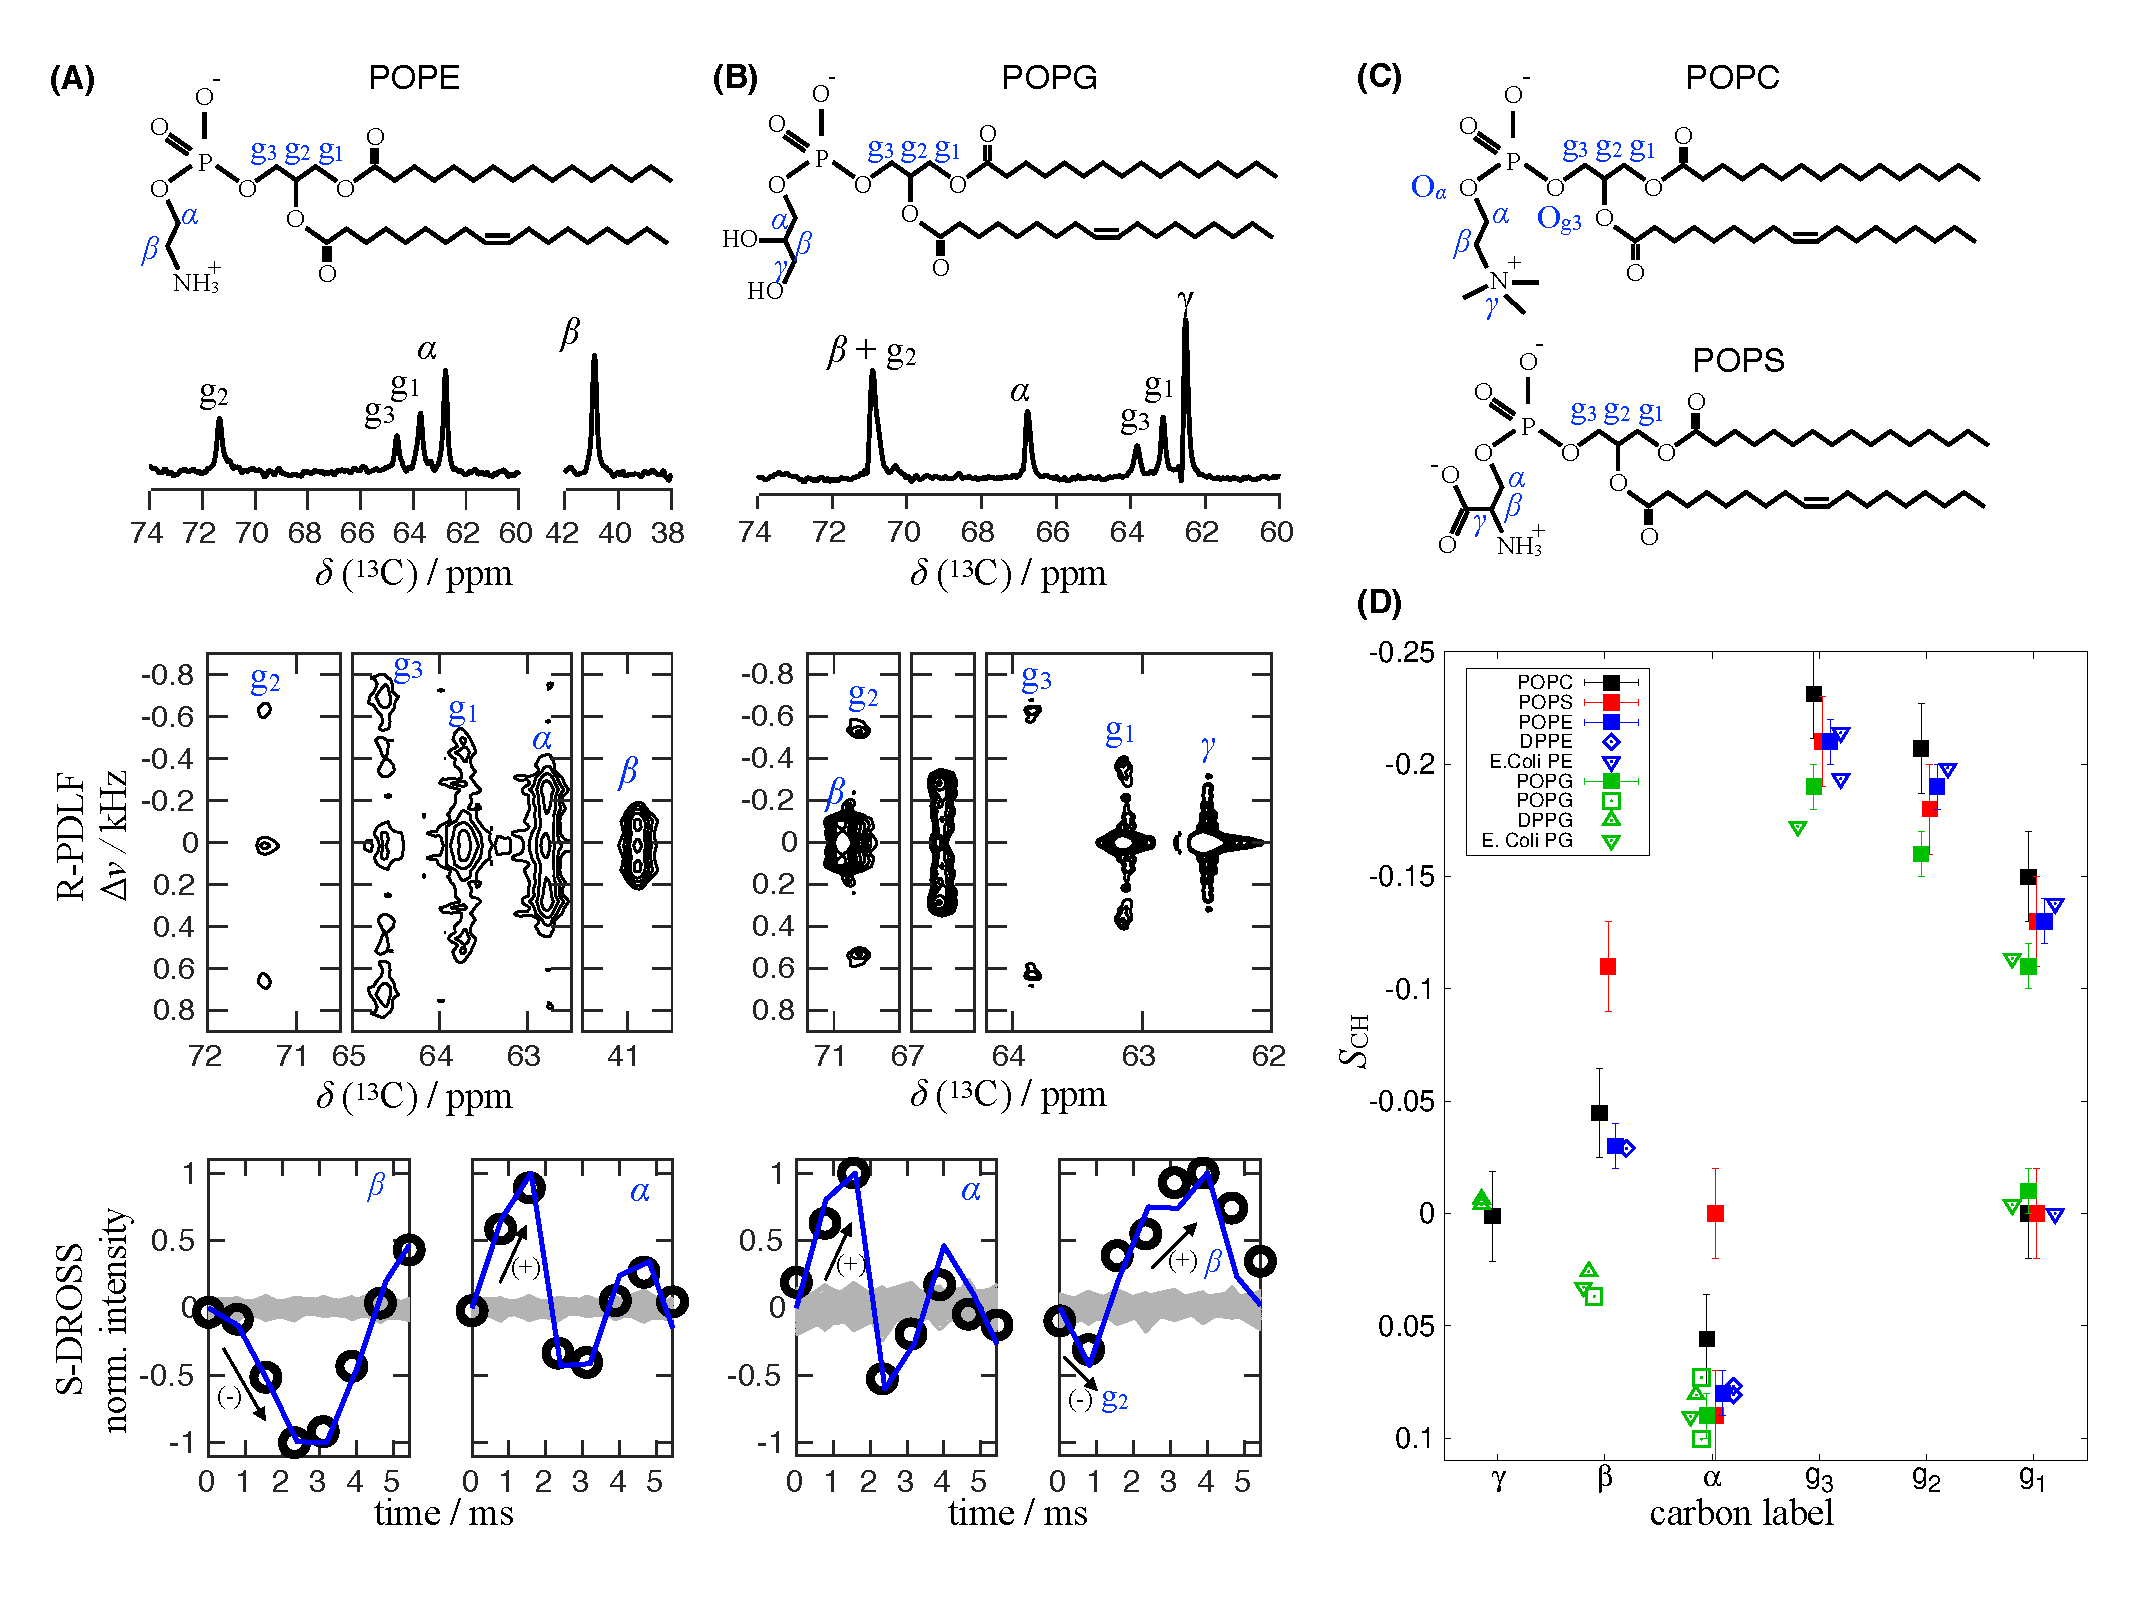
\includegraphics[width=\textwidth]{./Figs/figure_PG_PE.pdf}
   \caption{\label{HGorderParameters}
     Chemical structure, refocused-INEPT spectrum, 2D R-PDLF spectra, and S-DROSS dipolar slices (from top to bottom) for \textbf{A)} POPE  and \textbf{B)} POPG multi-lamellar vesicles measured by $^1$H-$^{13}$C solid-state NMR. The S-DROSS dipolar slices show both experimental data (open circles) and the result of NMR numerical simulations (blue solid lines).
     Full NMR spectra are shown in Figs. \ref{POPEspectra} and \ref{POPGspectra}.
     \textbf{C)} Chemical structure of POPC and POPS.
    \textbf{D)} Headgroup and glycerol backbone C--H bond order parameters $S_\mathrm{CH}$ for different phospholipids measured in the lamellar liquid disordered phase.
    Filled squares show $S_{\rm{CH}}$ magnitudes and signs determined by $^1$H-$^{13}$C NMR spectroscopy for POPE (310~K) and POPG (298~K), as
    measured in this work, and from data previously reported for POPS (298~K) \cite{antila19} and POPC (300~K) \cite{ferreira13,ferreira16}. Empty symbols show headgroup and glycerol backbone $S_{\rm{CH}}$ magnitudes measured previously with $^2$H NMR and are also plotted as real values using the signs determined in this work for 
    POPG with 10\,mM PIPES (298~K) \cite{borle85},
    DPPG with 10\,mM PIPES and 100\,mM NaCl (314~K) \cite{wohlgemuth80}, 
    DPPE (341~K) \cite{seelig76},
    {\it E. coli} PE and {\it E. coli} PG with 10\,mM PIPES and 100\,mM NaCl (310~K) \cite{gally81}.
   }
\end{figure*}


To experimentally characterize the differences in headgroup conformational ensembles of lipids that are not
bound to proteins, we measured the C--H bond order parameters $S_\mathrm{CH}$
and their signs of POPG and POPE in the liquid lamellar phase, as we did previously for POPC and POPS \cite{ferreira13,ferreira16,antila19}.
Determination of headgroup and glycerol backbone $S_\mathrm{CH}$ and their signs
was straightforward from the data in Figs.~\ref{HGorderParameters}, \ref{POPEspectra} and \ref{POPGspectra}
for all the C--H bonds, except for the $\beta$ and g$_2$ carbons in POPG.
These carbons have overlapping peaks in the INEPT spectra due to their similar chemical environments,
and only the magnitude of the larger order parameter could be determined from the R-PDLF spectra (Fig.~\ref{HGorderParameters}B).
Based on previous $^2$H NMR measurements \cite{wohlgemuth80,gally81,borle85},
we assigned the larger $S_\mathrm{CH}$ to the g$_2$ carbon
and used the literature value for the $\beta$-carbon in SIMPSON simulations to determine the signs.
The decrease in the beginning of the S-DROSS curve suggests that the sign of the larger g$_2$ $S_\mathrm{CH}$
is negative, and the later increase suggests that sign of the smaller $\beta$ $S_\mathrm{CH}$ is positive, as confirmed by the SIMPSON simulations (Fig.~\ref{HGorderParameters}B).

Experimental order parameters of POPC, POPE, POPG, and POPS glycerol backbones and headgroups from this and previous studies are displayed in Fig.~\ref{HGorderParameters}D, where the signs from $^{13}$C NMR experiments are used also for the $^2$H NMR data from the literature. The overall agreement of $S_\mathrm{CH}$ determined by different research teams and different techniques for the same lipid headgroup was excellent (within $\pm$0.02) here and in previous studies \cite{botan15,ollila16,antila19}. Therefore, the differences between lipid types are dictated by the headgroup chemistry rather than inaccuracies in experiments, or differences in the acyl chains or in the experimental conditions.


The most distinct order parameters are observed for PS headgroups, for which the $\alpha$-carbon $S_\mathrm{CH}$ exhibits significant forking (different values for different hydrogens bound to the same carbon) and the $\beta$-carbon has a more negative value than in other studied lipid types. On the other hand, the $\beta$-carbon $S_\mathrm{CH}$ of PG headgroup has a positive sign, in contrast to all the other lipid types. The sign has not been previously known from $^2$H NMR experiments which enable detecting only order parameter absolute values~\cite{wohlgemuth80,gally81,borle85}. The glycerol backbone order parameters are similar for all the lipid types, although they move slightly toward positive values (closer to zero) in the order PC $<$ PE $<$ PS $<$ PG. Only minor differences between PC and PE headgroups are observed.

\subsection{Conformational ensembles of different lipid headgroups from MD simulations}

\begin{figure*}
  \centering
   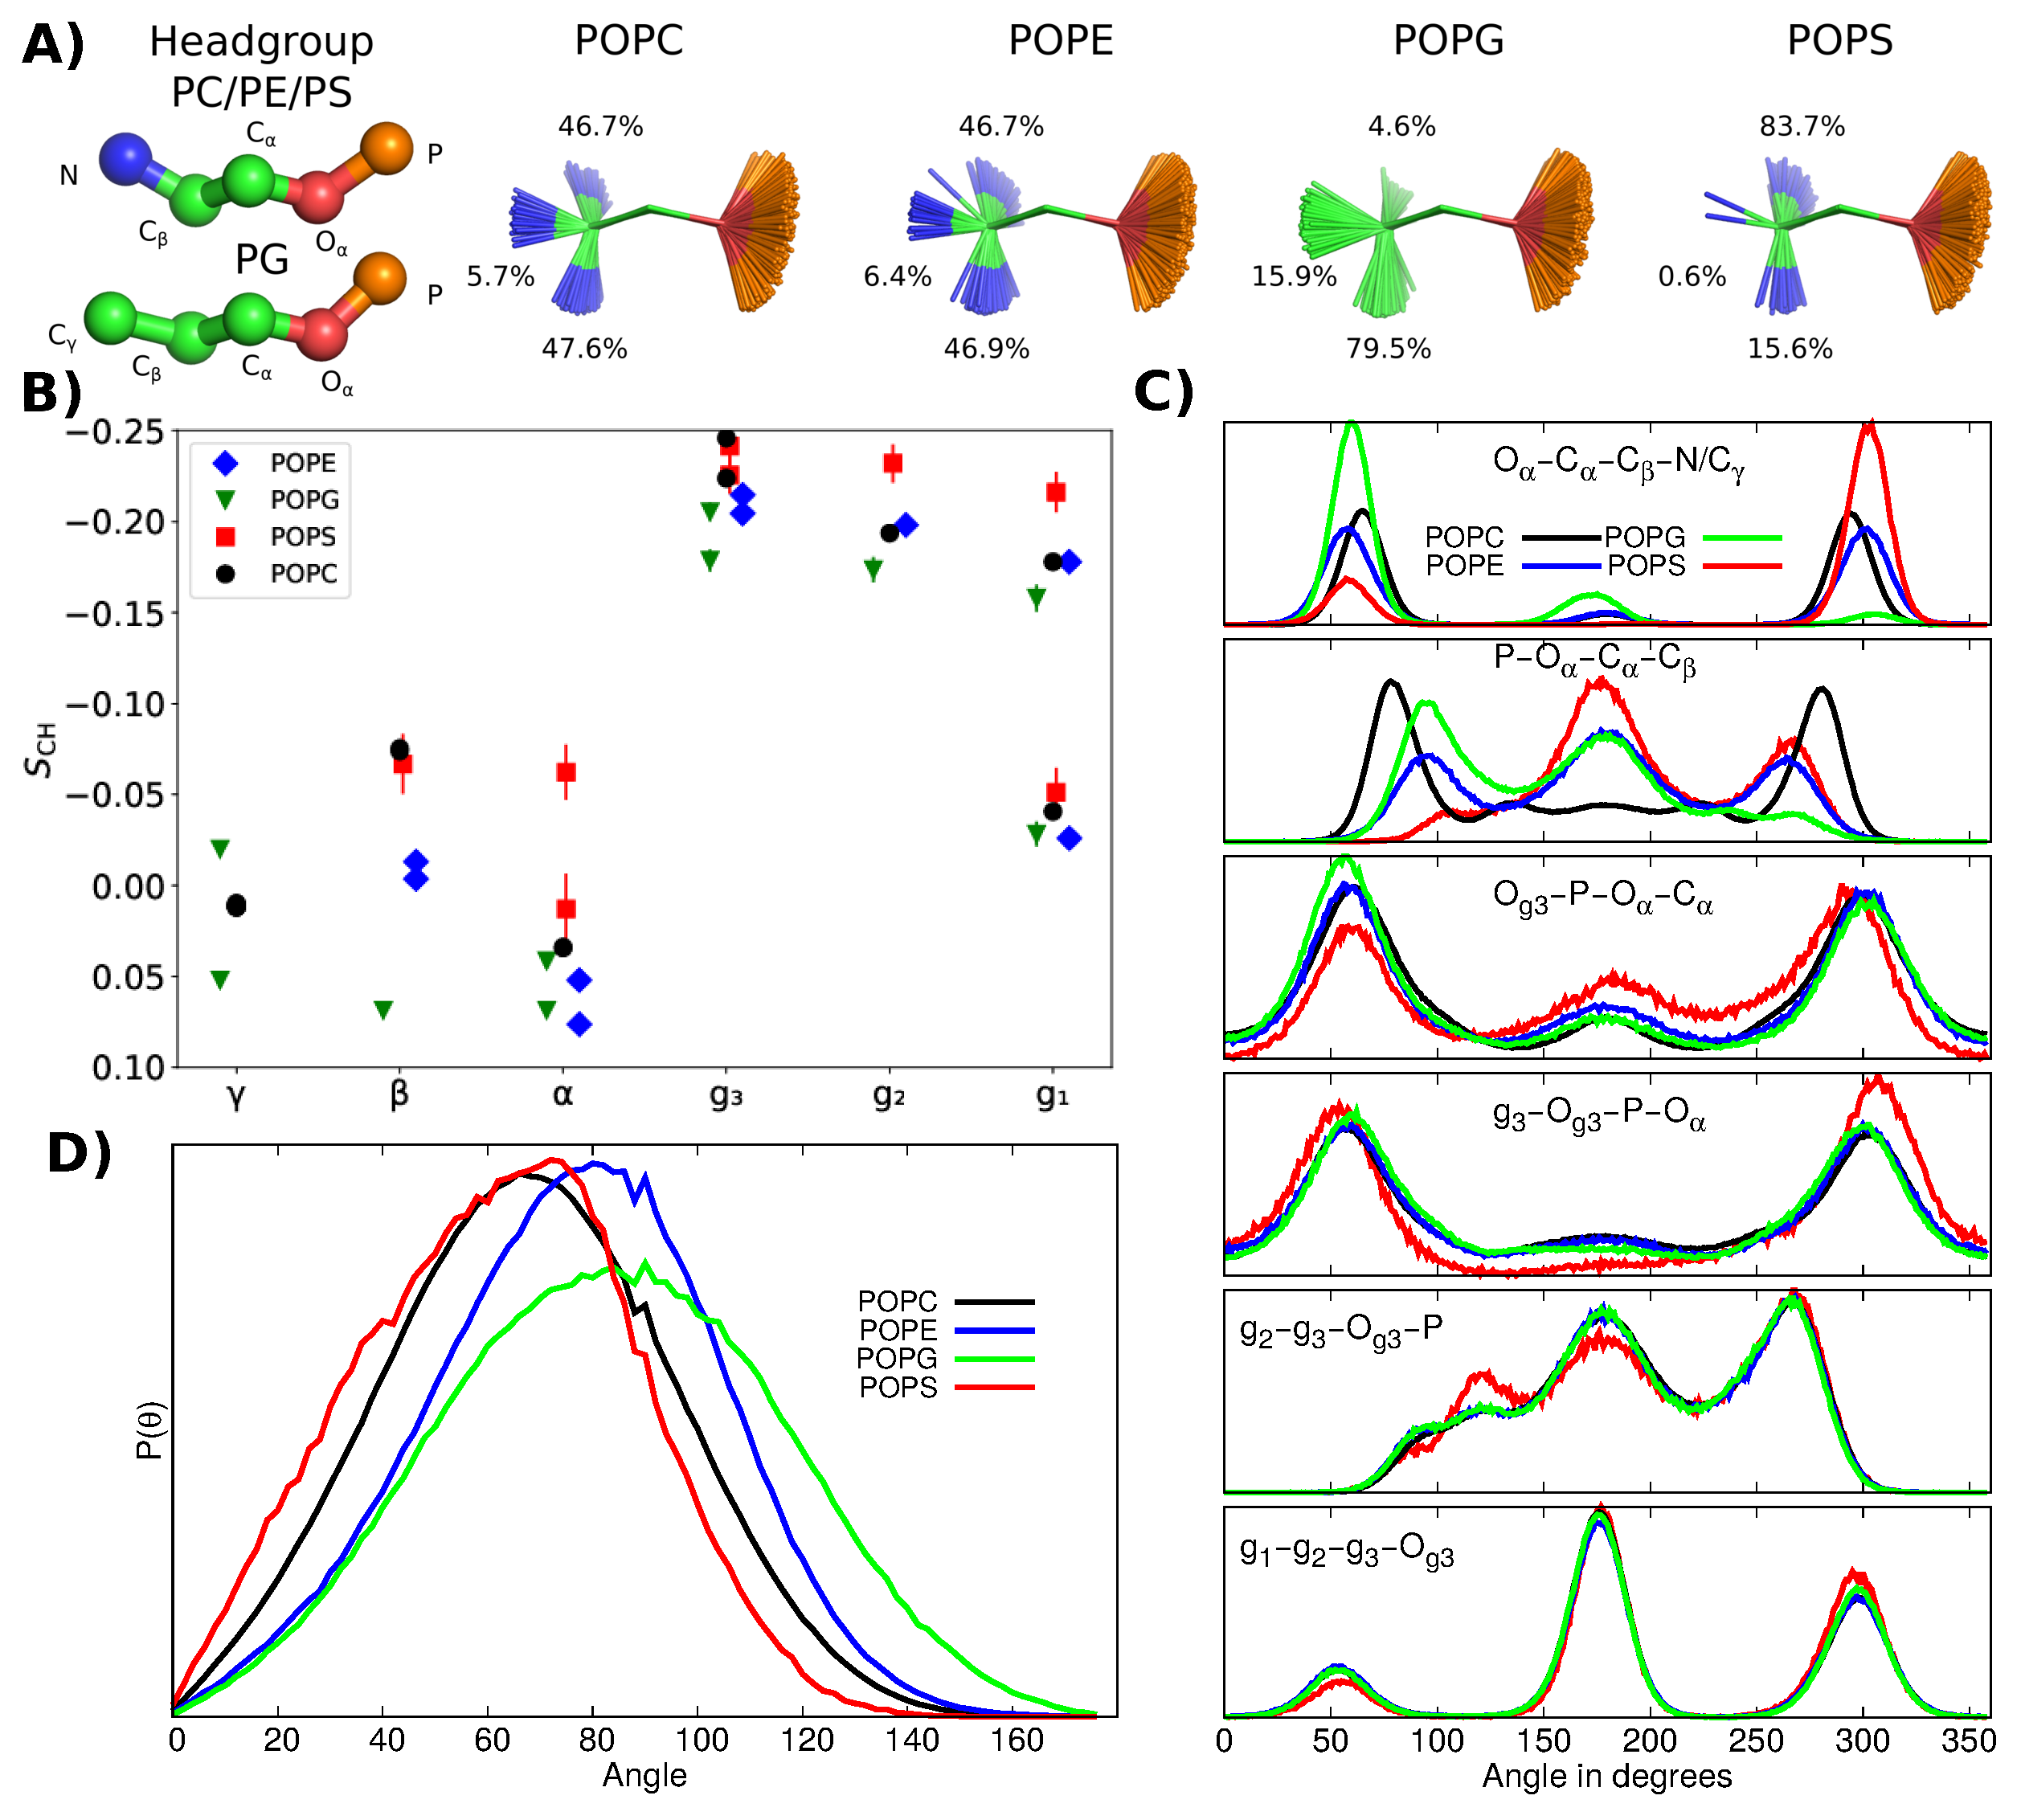
\includegraphics[width=\textwidth]{./Figs/figure2.eps}
   \caption{\label{structures}
     Results from the best simulation model demonstrating the differences in conformational ensembles between different lipid types.
     The best simulation model (CHARMM36) was selected from the comparison of ten different force fields based on quality evaluation against experimental $S_{\rm{CH}}$ values in Figs.~\ref{HGorderParametersPE} and~\ref{HGorderParametersPOPG}.
     \textbf{A)} Snapshots with overlayed C$_\beta$, C$_\alpha$ and O$_\alpha$ atoms and occurrence of different conformations.
     \textbf{B)} Headgroup and glycerol backbone region order parameters of the different lipid types. Colored shaded regions show the range of experimental values from Fig. \ref{HGorderParameters}.
     \textbf{C)} Relative free energies for individual heavy atom dihedral angles estimated from the inverse Boltzmann formula.
     Angles corresponding to free energies above 8~$k_\mathrm{B}T$ are not shown because they are not observed in simulations.
     \textbf{D)} Distributions of the P--N/C$_\gamma$ vector angle with respect to the membrane normal.
  }
\end{figure*}

Ideal
MD simulations would correctly predict the conformational ensembles of lipids, thereby giving an interpretation for  the experimental C-H bond order parameters, $S_\mathrm{CH}$, due to their direct connection~\cite{ollila16}. To find the best MD simulation models (force fields) for this purpose, we took advantage of the power of the NMRlipids Project, an open science collaboration that has gathered a massive number of simulation trajectories, allowing the evaluation of all the available force fields of PC~\cite{botan15}, PS~\cite{antila19}, PE (Fig.~\ref{HGorderParametersPE}), and PG (Fig.~\ref{HGorderParametersPOPG}) lipids against NMR data. The comparison of hundreds of simulation trajectories simulated with approximately 20 different force fields revealed that none of them can correctly capture the lipid conformational ensembles and reproduce the experimental $S_\mathrm{CH}$ of all segments within experimental error (for detailed discussion on the quality of force fields, see section S3 in the supplementary information and Refs. \citenum{botan15,ollila16,antila19,antila21a}). However, CHARMM36, the force field showing the best agreement with experiments, correctly captures the essential differences between the PC, PE, PG, and PS headgroup order parameters, particularly the positive order parameter of $\beta$-carbon in PG and the forking of $\alpha$-carbon in PS, see Fig.~\ref{structures} B. 

To understand the structural origin of distinct order parameters for the distinct lipids,
we first calculated and visualized the heavy atom dihedral angle distributions from the best performing simulations that reproduced the differences between headgroups~(Figs.~\ref{structures} B and \ref{DIHdists}).
Then, we used the inverse Boltzmann formula to estimate the free
energy costs for different dihedral angle orientations.
The results in Fig.~\ref{structures}C suggest that all lipid headgroups are very flexible and free
energy costs for rotating individual dihedrals to almost any angle is low (below 8~$k_\mathrm{B}T$).
Only $cis$ states of P-O$_\alpha$-C$_\alpha$-C$_\beta$ and g$_2$-g$_3$-O$_{g_3}$-P have larger relative free
energies and are not observed for any lipids during the simulations.


Major differences between headgroups are observed for the last two dihedrals in the headgroup end,
O$_\alpha$-C$_\alpha$-C$_\beta$-N/C$_\gamma$ and P-O$_\alpha$-C$_\alpha$-C$_\beta$,
which prefer \textit{gauche$^-$} conformations for PG and \textit{gauche$^+$} for PS,
whereas PC and PE exhibit symmetric distributions.
Also, the free energy barriers for O$_\alpha$-C$_\alpha$-C$_\beta$-N/C$_\gamma$ dihedral
rotations between \textit{gauche} and \textit{trans} states are larger for
PS and PG lipids than for PC and PE lipids. 
The rest of the dihedrals are similar between different lipids,
with the exception of PS lipids for which slightly larger free energy for \textit{eclipsed anti} conformation
in g$_3$-O$_{{\mathrm g}3}$-P-O$_\alpha$ dihedral was observed.
Therefore we suggest that the main differences between lipid headgroups leading to distinct order parameters occur in the headgroup end, while in the phosphate region they remain similar in different lipids with the exception of PS. The increased barriers for dihedral rotations may explain the more rigid headgroup structures in PS~\cite{browning80,buldt81}. Furthermore, the angle between headgroup dipole and membrane normal decreases in the order of PG $>$ PE  $>$ PC  $>$ PS (Fig.~\ref{structures}D). However, the differences between PC and PE in P-O$_\alpha$-C$_\alpha$-C$_\beta$ dihedral
and P--N vector dipole may be artificial as the $\beta$-carbon order parameter in PC is too negative even in the best available force field~ \cite{botan15}, thereby not being equal to the order parameter in PE as observed in experiments.

In conclusion, the rotation of dihedral angles to almost any position bears relatively low free energy cost and the sampled dihedral angles are within similar ranges for all studied headgroup types. In other words, all studied lipid headgroups sample very broad conformational ensembles in the liquid lamellar phase. Therefore, the lipid headgroups are able to adopt a wide range of conformations when interacting with proteins, ions, or other biomolecules. Furthermore, the structures in lipid crystals \cite{buldt81,pascher92} are not representative of the liquid state, and models aiming to explain NMR data using only a few conformations \cite{seelig77c,davis83,Semchyschyn04,akutsu20} are not sufficient to capture the large conformational space of lipids in the liquid lamellar state.
However, conformational ensembles of lipids in MD simulation trajectories with accurate force fields that capture the experimental NMR order parameters can be considered realistic, and thereby used to interpret the experimental data.


\subsection{Lipid conformational ensembles in charged membranes}



\begin{figure*}[bt]
  \centering
  \includegraphics[width=\textwidth]{./Figs/HGorderparametersPCvsSURFchangeDIHEDRALSlog.eps}
  \caption{\label{changesWITHsurf}
    \textbf{A)} Modulation of PC headgroup order parameters and P--N vector tilt (average angle between the P-N vector and the bilayer normal) upon addition of cationic surfactant (dihexadecyldimethylammonium)
    from CHARMM36 simulations compared with the experimental data \cite{scherer89}.
    \textbf{B)} Relative free energies for individual dihedral angles estimated from inverse Boltzmann distributions of heavy atom dihedral angles
    with different amounts of cationic surfactant from CHARMM36 simulations.
  }
\end{figure*}



Charged entities, such as lipids, proteins, surfactants, drugs, and ions incorporated in membranes can change the orientation of the headgroup dipole in PC lipids and affect the order parameters of the lipid headgroups~\cite{seelig87}. However, the detailed understanding of the structural and energetic responses of lipids to membrane-bound electric charge is still lacking \cite{Semchyschyn04}. For example, it is not clear if the membrane-bound charges restrain the lipids into specific conformations or just redistribute the probabilities of states by keeping the accessible conformations similar. 

To resolve lipid headgroup conformational ensembles in cellular membranes bearing positive charge,
we calculated the heavy atom dihedral angle distributions from 
the subset of simulations 
that correctly captured the experimentally measured decrease in PC headgroup order parameters upon addition of cationic surfactants into a bilayer (figure \ref{changesWITHsurf} A).
The dihedral angle distributions and relative free energies
in figures \ref{HGorderparametersPCvsSURFdihedrals} and \ref{changesWITHsurf} B reveal that the
addition of positive charge into a membrane 
decreases the abundance of \textit{trans} states in g$_2$-g$_3$-O$_{g_3}$-P and g$_3$-O$_{g_3}$-P-O$_\alpha$, and \textit{cis} states in O$_{g_3}$-P-O$_\alpha$-C$_\alpha$ dihedrals.
The choline region remains essentially unchanged and only minor changes are observed in the other dihedrals even at a surfactant molar fraction of 0.47.

In addition, binding of ions to the membrane may affect the lipid headgroup conformational ensembles under physiological conditions.
The bound Ca$^{2+}$ ion to PC headgroup leads to similar decrease in trans state probability for g$_3$-O$_{g3}$-P-O$_\alpha$ dihedral
in the most realistic MD simulation models
as observed for cationic surfactants
(lipid17ecc and CHARMM36 in Figs.~\ref{DIHSwithCAlipid17eccPOPC}, \ref{DIHSwithCAcharmm36POPC} and Fig.~\ref{changesWITHCaClPG}).
The dihedral distributions of the PG headgroup are more sensitive to the bound ions in the most realistic simulations,
but upward tilting of the headgroup dipole upon the addition of CaCl$_2$ is weaker than in PC
(Lipid17 and Slipids in Figs.~\ref{changesWITHCaClPG},~\ref{DIHSwithCAslipidsPOPG} and \ref{DIHSwithCAlipid17POPG}).
However, the changes in PG lipid dihedrals upon the addition of CaCl$_2$ differ between the best models (Figs.~\ref{DIHSwithCAslipidsPOPG} and~\ref{DIHSwithCAlipid17POPG}), and none of the simulations captures the Ca$^{2+}$ ion binding affinity and conformational ensemble of PG lipids simultaneously. Moreover, experimental data to evaluate the response of $\alpha$-carbon order parameters to the added CaCl$_2$ in PG is not available.
Additionally, the headgroup conformational ensembles in mixtures of PC and charged (PG or PS) or zwitterionic (PE)
lipids could not be resolved with the currently available force fields and experimental data
(Figs.~\ref{HGorderparametersPCvsPEPG} and~\ref{HGorderparametersPGvsPCchange}, and Ref.~\cite{antila19,melcr20}).

In conclusion, the MD simulation results suggest that the structural response of lipid headgroups to 
membrane-bound charges arises
from mild changes in dihedral angle distributions, rather than restriction of lipids to
fixed conformations. Therefore, lipid headgroups sample a large space of different conformations
also in charged membranes, thereby retaining the capability to adopt multiple conformations when
interacting with proteins or other molecules.



\subsection{Protein-bound lipid conformations}

\begin{figure*}[tb]
  \centering
  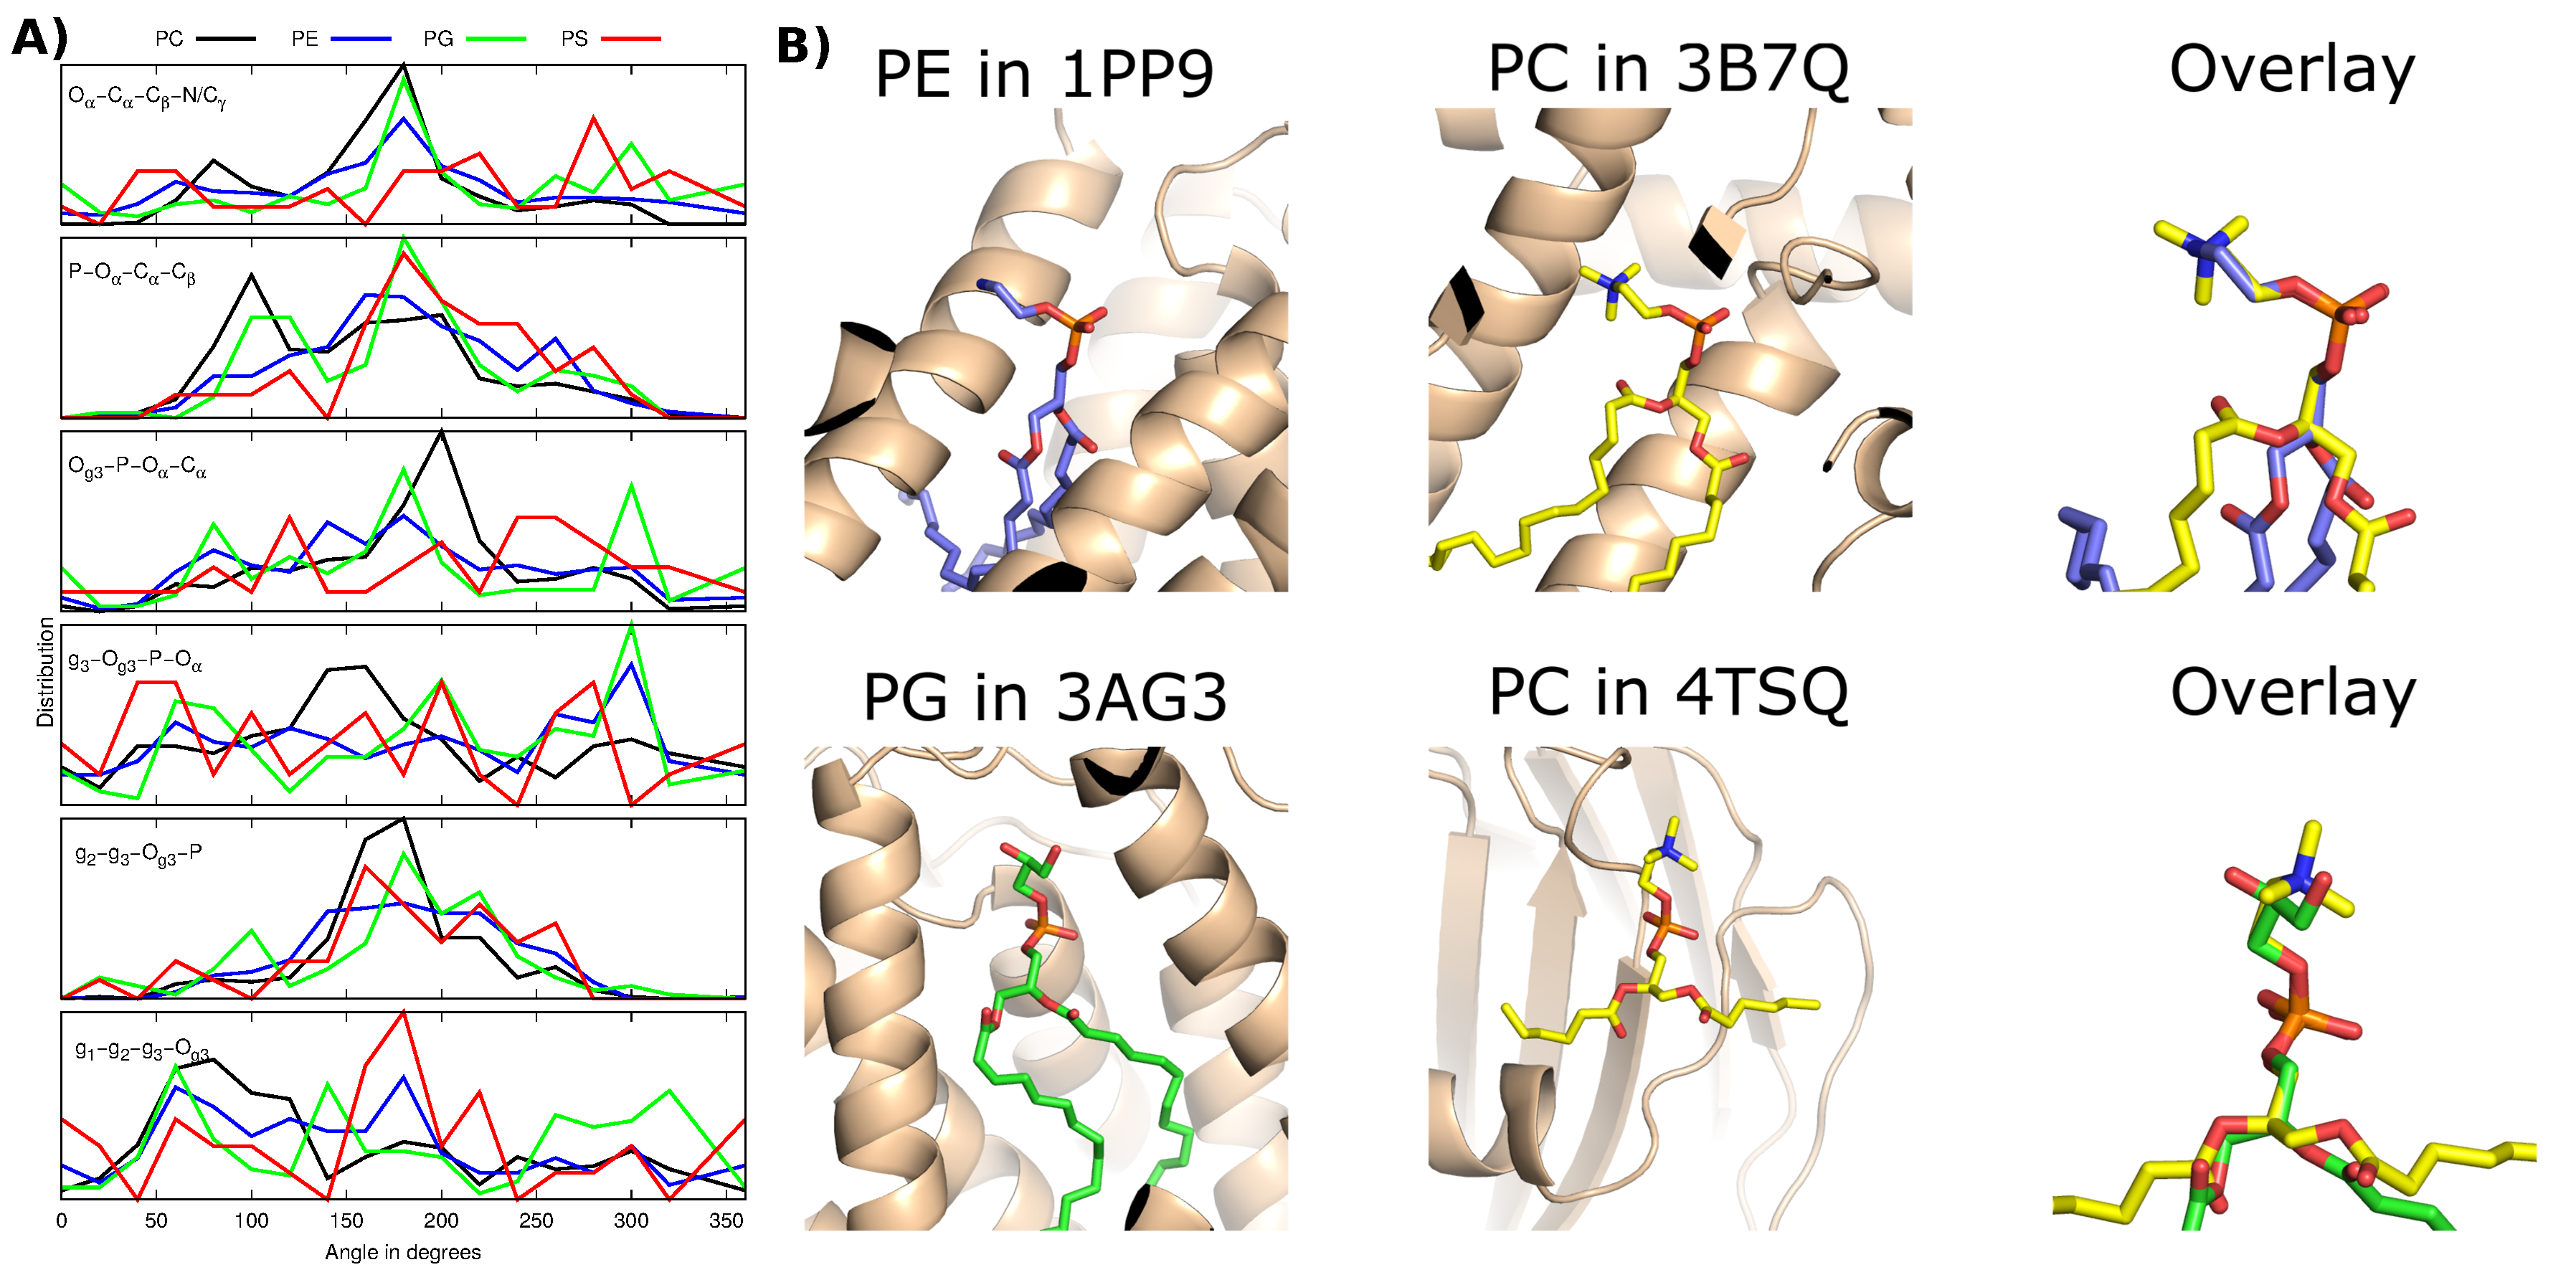
\includegraphics[width=\textwidth]{./Figs/figure4.eps}
  \caption{\label{dihedralsFROMpdb}
    A) Heavy atom dihedral angle distributions calculated from lipid structures in PDB.
    B) The structure of PE headgroup bound to cytochrome {\it bc}$_1$ complex (PDB ID: 1PP9 \cite{huang05})
    with identical conformation as the PC headgroup bound to yeast Sec14 (PDB ID: 3B7Q \cite{schaaf08}),
    and the structure of PG headgroup bound to bovine cytochrome {\it c} oxidase (PDB ID: 3AG3 \cite{muramoto10})
    with identical conformation as PC to FraC, a pore-forming toxin (PDB ID: 4TSQ \cite{tanaka15}).
  }
\end{figure*}


Interpretation of experimental order parameters using MD simulations
in previous sections suggest that PC, PE, PG, and PS lipid headgroups are very flexible,
allowing them to bind proteins in various different conformations.
To test this prediction, we analyzed the conformations of all protein-bound lipids 
from structures deposited in the PDB \cite{berman00}.
We found 311 PC, 394 PE, 154 PG, and 35 PS lipid conformations that were bound to different types of proteins 
(including both integral and peripheral membrane proteins) and were determined as a part of protein structure using crystallography or cryo-EM. The full list of structures with bound lipids is available from {\it Data/PDBdistributions/pdbtable.pdf} in Ref.~\cite{NMRlipidsIVbgit}.

The heavy atom dihedral angle distributions calculated from these conformations 
(Fig.~\ref{dihedralsFROMpdb} A) reveal that the protein-bound lipids indeed exhibit a wide
range of conformations, independent of the headgroup type.
As for bulk lipid bilayers (Figs.~\ref{structures}C, \ref{DIHdists}), only {\it cis} conformations
of P-O$_\alpha$-C$_\alpha$-C$_\beta$ and g$_2$-g$_3$-O$_{g_3}$-P dihedrals are almost
completely absent in all lipids, and significant differences between
different headgroups are not observed.
Deviation of protein-bound lipid structures from protein-free lipid structures in crystals 
has been previously proposed to indicate inaccuracies in lipid structures in PDB \cite{marsh13b,pezeshkian18}. 
However, we observe large deviations from the protein-free lipid crystal structures also in conformational ensembles
that reproduce the NMR data in the liquid lamellar phase, indicating that such deviations
are realistic also in the protein-bound states.


Our results suggest that flexible lipid headgroups can optimize the intermolecular interactions with proteins by binding
in a wide range of conformations.
Therefore, the specific binding of lipids to proteins is not driven by differing structural preferences between headgroups.
This is demonstrated in Fig.~\ref{dihedralsFROMpdb} B with two examples where different lipid types bound to
different proteins have almost identical headgroup conformations:
PE in cytochrome {\it bc}$_1$ complex is similar to PC bound to yeast Sec14,
and PG bound to bovine cytochrome {\it c} oxidase is similar to PC bound to pore-forming toxin (FraC).
On the other hand, a single lipid headgroup type is capable of accommodating various binding positions and as such would 
be able to specifically bind to many different kinds of binding sites.


\section{Conclusions}

C--H bond order parameters $S_\mathrm{CH}$ from NMR experiments 
suggest that lipid headgroup conformational ensembles depend on lipid type (PC, PE, PG, or PS) 
and membrane charge (cationic lipids, surfactants, accumulated ions or drugs). 
Our analysis of these data, using MD simulations collected
within the NMRlipids Project,
revealed that the differences in $S_\mathrm{CH}$ can be explained
by small changes in the dihedral angle probability distributions.
All four studied headgroup types (PC, PE, PG, and PS) are flexible
and access a similarly wide range of conformations, with very few restrictions in dihedral orientations---also when membranes are charged.
In conclusion, the observed differences in $S_\mathrm{CH}$ originate from
slightly reweighed conformational probabilities rather than changes in accessible structures.

The flexibility and wide conformational space of headgroups suggest that protein--bound lipids can
adapt to various binding sites to optimize the lipid--protein interactions.
We tested this prediction by analyzing from PDB the conformations of lipids that are tightly bound to proteins.
We found that also the protein-bound lipids exhibit a wide range of conformations, without significant 
differences between different lipid types: The specificity of lipid binding to proteins is not
regulated by accessible lipid structures, but a single lipid type can adapt to various binding pockets.

Our results suggest that lipid headgroup binding to proteins can be described by the {\it inverse conformational selection model}
where unbound lipids sample a wide conformational ensemble offering the large selection of conformations
that can bind to various binding sites in substrates, such as protein, drug, RNA, or virus, that remain conformationally fixed.
In this model, the binding energy is dominated by
intermolecular interactions and changes in lipid conformational entropy, while 
conformational restrictions inherent to the lipids play a minor role.
Here we have focused only on lipid headgroups while potential applications of the proposed model on interactions between hydrophobic acyl chains and proteins are left for future studies. 
Applications of the proposed model in molecular cell biology include the understanding of lipid-mediated cell signaling
and functions of lipid regulated membrane proteins in general. 
In bionanotechnology, our model facilitates, for example,
the design of phoshopolipid-specific antibodies and lipid nanoparticle carriers with minimal sides effects for mRNA vaccines.
Furthermore, our work has demonstrated the power of open access MD simulation data
to complement the PDB data in elucidating behavior of complex systems of disordered biomolecules.

\section{Methods}
\subsection{Experimental C--H bond order parameters}
The headgroup and glycerol backbone C--H bond order parameters of 1-palmitoyl-2-oleoyl-sn-glycero-3-phosphoethanolamine (POPE) and 1-palmitoyl-2-oleoyl-sn-glycero-3-phospho-(1'-rac-glycerol) (POPG), purchased from Avanti polar lipids, were measured using natural abundance $^1$H-$^{13}$C solid state NMR spectroscopy as described previously \cite{ferreira13,ferreira16}. The samples were prepared by simply mixing the lipids with water until a homogeneous preparation of multi-lamellar vesicles (MLVs) was attained and left to equilibrate for approximately 24 hours before measurements. The magnitudes of the order parameters were determined using a R-type Proton Detected Local Field (R-PDLF) experiment~\cite{dvinskikh04}, and the order parameter signs from S-DROSS experiments~\cite{gross97} combined with SIMPSON simulations \cite{bak00}.
%The experiments were done in a Bruker Avance III 400 spectrometer operating at a $^1$H Larmor frequency of 400.03 MHz.
%Magic angle spinning (MAS) of the sample was used at a frequency of 5.15 kHz (R-PDLF experiment) and 5 kHz (S-DROSS experiment).
The set-up of the solid-state NMR experiments were identical as in our previous work~\cite{antila19}. The POPE experiments were recorded at 310~K and POPG experiments at 298~K, where the bilayers are in the liquid disordered phase \cite{marsh13}.

Glycerol backbone peaks from both lipids, and the $\alpha$-carbon peak from POPE in the INEPT spectra 
were assigned based on previously measured POPC spectra~\cite{ferreira13}.
The $\beta$-carbon peak from POPE was assigned based on $^{13}$C chemical shift table for amines available
at \url{https://www.chem.wisc.edu/areas/reich/nmr/c13-data/cdata.htm}. The asignment of the $\alpha$, $\beta$, and $\gamma$ peaks of POPG was based on the measured R-PDLF dipolar couplings in comparison to the known order parameters from previous $^2$H\,NMR experiments~\cite{borle85,wohlgemuth80}.   
The $\beta$-carbon peak from POPG overlapped with the g$_2$ peak from glycerol backbone
because their chemical environments are similar.

\subsection{Molecular dynamics simulations}

Molecular dynamics simulation data were collected and analyzed using
the methods from the NMRlipids Open Collaboration project (\url{nmrlipids.blogspot.fi}) \cite{botan15,catte16,ollila16,antila19}.
Simulation details, accessibility information and quality evaluation of approximately 70 combinations of lipid headgroup and force field simulated for this work are in the supplementary information.

Best models for the interpretation of lipid headgroup conformational ensembles from the experimental data were selected
using quality evaluation measures defined in the NMRlipids project.
Conformational ensembles of headgroup and glycerol backbone in PE and PG simulations were evaluated using the C--H bond order parameters \cite{botan15}. Interactions between different headgroups were evaluated by monitoring the changes in headgroup order parameters upon mixing the lipids \cite{antila19}. The ion binding affinities and response of lipids to bound charge were evaluated by monitoring the changes in lipid headgroup order parameters \cite{catte16,antila19}.

The differences in headgroup conformation ensembles were analyzed calculating the distributions of six dihedral angles, O$_\alpha$-C$_\alpha$-C$_\beta$-N/C$_\gamma$, P-O$_\alpha$-C$_\alpha$-C$_\beta$, O$_{g3}$-P-O$_\alpha$-C$_\alpha$, g$_3$-O$_{g3}$-P-O$_\alpha$, g$_2$-g$_3$-O$_{g3}$-P, and g$_1$-g$_2$-g$_3$-O$_{g3}$, labeled in Fig. \ref{HGorderParameters} C. Relative free energy costs for turning dihedral angles with respect to the most probable value (lowest free energy) were estimated from the inverse Boltzmann formula $\Delta E(\theta) = -kT \left[\ln\left[p(\theta)\right]-\ln\left[p(\theta_0)\right] \right]$, where $p(\theta)$ is the dihedral angle distribution and $\theta_0$ is the most probable angle from MD simulation.

\subsection{Analysis of protein-bound lipid conformations}
Lipid structures from the Protein Data Bank (PDB, \cite{berman00})
were searched using PDBe REST API (\url{www.ebi.ac.uk/pdbe/pdbe-rest-api})
using the ligand names listed in the supplementary information.
Dihedral distributions from the lipid structures were calculated
using the MDAnalysis Python library \cite{agrawal11,gowers16} and
Jupyter notebook available from {\it scripts/PDBanalysis.ipynb} folder in Ref~\citenum{NMRlipidsIVbgit}.
Only the structures determined using X-ray crystallography or Cryo-EM with a resolution higher than 3.2~\text{\AA} were used in the analysis. Some structures of multimeric proteins contained multiple lipids in the same conformation. The conformations were considered identical if all dihedral angles were the same within 3 degrees. In these cases, this conformation was counted only once for the subsequent analyses
to avoid its overweighting.
  
To demonstrate the existence of similar structures of different lipids bound to different proteins, we searched for pairs having the last five heavy atom dihedrals angles in the headgroup end (excluding g$_1$-g$_2$-g$_3$-O$_{g3}$ from the list in previous section) within
30 degrees of each other among the structures with resolution higher than 2.5~\text{\AA}. The two most representative examples
were handpicked from the results.

\begin{suppinfo}

Additional NMR data, ligand names in PDB used to analyse the protein--bound lipid conformations, evaluation of MD simulations against NMR experiments, dihedral angle distributions from simulations, and description of simulated systes with simulation details. 

%This will usually read something like: ``Experimental procedures and
%characterization data for all new compounds. The class will
%automatically add a sentence pointing to the information on-line:

\end{suppinfo}


\begin{acknowledgement}

  % Put your acknowledgments here.
A.P. is grateful to the Centro de
Supercomputaci{\'o}n de Galicia (CESGA) for use of the Finis
Terrae computer.
M.J. thanks CSC -- IT Center for Science for computational resources and the Emil Aaltonen foundation for financial support.
T.M.F. was supported by the Ministry of Economics, Science
and Digitalisation of the State of Saxony-Anhalt, Germany.
P.B. was supported by the Academy of Finland (Grant 311031).
F.F.-R. acknowledges Tecnol\'{o}gico Nacional de M\'{e}xico Proyecto IT16C431, Direcci\'{o}n General de Asuntos del Personal Acad\'{e}mico (DGAPA) Programa de Apoyo a Proyectos de Investigaci\'{o}n e Innovaci\'{o}n Tecnol\'{o}gica (PAPIIT) IG100920, CONACyT Ciencia de Frontera 74884 for financial support and Miztli-Direcci\'{o}n de C\'{o}mputo y de Tecnolog\'{i}as de Informaci\'{o}n y Comunicaci\'{o}n (DGTIC) - Universidad Nacional Aut\'{o}noma de M{\'e}xico (UNAM) (Project LANCAD-UNAM-DGTIC-057) facilities for computing-time allocation.
I.G. was supported by the Ministry of Science and Higher Education of the Russian Federation (agreement \#075-00337-20-03, project FSMG-2020-0003). 
J.J.M. gratefully acknowledges financial support from the Carlsberg 
Foundation in the form of a postdoctoral fellowship while at 
the University of Chicago (grants CF15-0552, CF16-0639, and 
CF17-0783) and the research framework provided by the 
Research Computing Center at the University of Chicago.
O.H.S.O, A.M.K, and S.I.V acknowledge CSC -- IT Center for Science for computational resources and Academy of Finland (grants 315596 and 319902) for financial support.
T.J.P. acknowledges use of the Iridis high-performance computing resources at the University of Southampton.
J.M. thanks the Center for Information Technology of the University of Groningen for their support and for providing access to the Peregrine high performance computing cluster.

\end{acknowledgement}


% Create the reference section using BibTe
\bibliography{refs.bib}


\end{document}
